
\section{Enhancing Bitcoin privacy}
There are basically two approaches for enhancing users privacy in Bitcoin:
\begin{itemize}
  \item Mixing services: they achieve users privacy generally without degrading
  the performance of the system. However, they require absolute trust in a third
  party.
  \item Cryptograpic extensions of Bitcoin: extensions of the Bitcoin protocol
  which eliminate the need for trusted third parties but tend to be less efficient
  in terms of performance.
\end{itemize}


%%%%%%%%%%%%%%%%%%%%%%%%%%%
% *** FIRST SUB-SECTION ***
%%%%%%%%%%%%%%%%%%%%%%%%%%%
\subsection{Mixing services} A bitcoin mixing service act as mediators and
provides anonymity by transferring payments from an input set of bitcoin
addresses to an output set of bitcoin addresses, such that is it hard to trace
which input address paid which output address, as schematized in figure
\ref{fig:mixing-service-scheme}. Examples of this kind of mixing services are
Mixcoin and CoinParty. The former relies on a third party can violate users
privacy and steal users’ bitcoins (theft is detected but not prevented), while
the second uses more mixing parties and it is considered secure only if $2/3$ of
the mixing parties are honest.

There is also another kind of mixing services in which the service acts as a
``coin hisory resetter''. In this case the user sends to the mixer a certain
amount of bitcoin and a return address and the mixer sends back to the user (to
the specified address) someone else’s coins of the same value. Examples of this
kind of services are BitLaundry and Bitcoin Fog. The problem of these services is
that they do not protect form network-layer attacks since the eventually the
user is the one making payments (instead of the mixing service).

\begin{figure}[!htb]
	\centering
	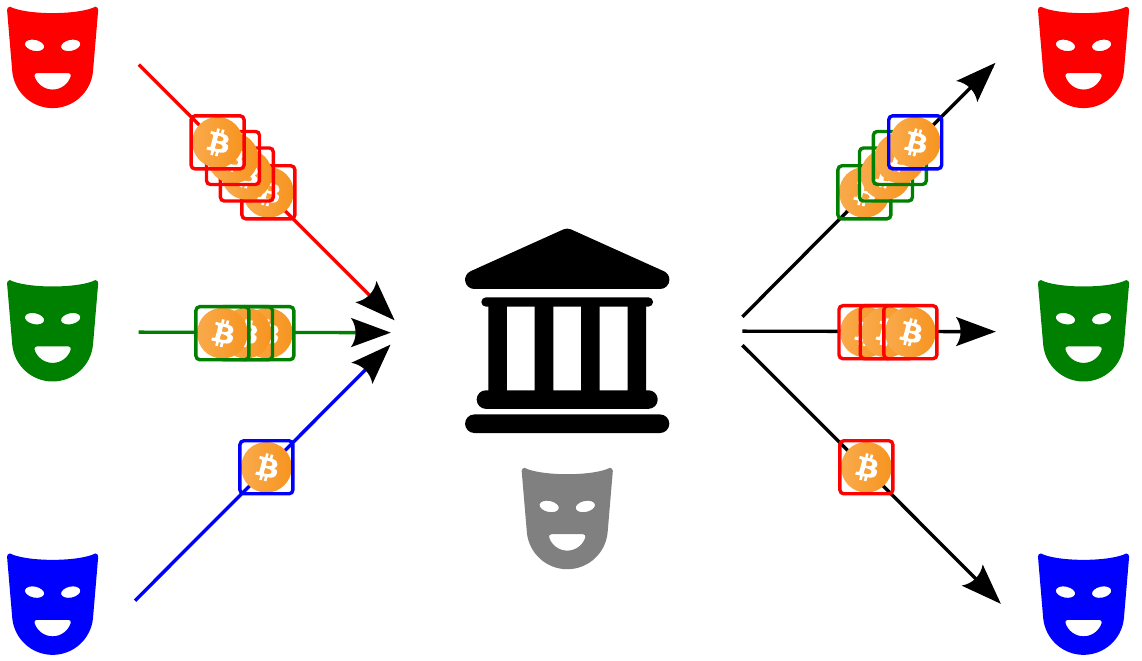
\includegraphics[width=1\linewidth]{img/mixing-service-scheme.png}
	\caption{Scheme of how a mixing service works}
	\label{fig:mixing-service-scheme}
\end{figure}






%%%%%%%%%%%%%%%%%%%%%%%%%%%
% *** SECOND SUB-SECTION ***
%%%%%%%%%%%%%%%%%%%%%%%%%%%
\subsection{Enhancing privacy through blind signatures} In the following section
is presented a mixing service scheme for enhancing Bitcoin privacy through the
use of blind signatures. The scheme has been proposed  by E. Heilman, F.
Baldimtsi and S. Goldberg \cite{heilman-blindly-signed-contracts}, is based on
the scheme used in eCash \cite{Chaum1984} and, unlike other previous schemes
that are efficient but achieve limited securit/anonymity or other which that
provide strong anonymity but are slow and require large numbers of transactions,
it provides anonimity at reasonable speed using an untrusted third party (which
can therefore be malicious).

\subsubsection{High-level overview of the scheme}
The scenario is the following: $A$, \emph{the payer}, wants to anonymously send
1 bitcoin to $B$, \emph{the  payee}. If $A$ performed a standard transaction
sending 1 BTC from $address_A$ (owned by $A$) to a fresh ephemeral address
$address_B$ (owned by $B$), there would be a record in the blockchain linking
the two addresses. Even if $A$ and $B$ always create a fresh address for each
payment they receive, the links between addresses can be used to de-anonymize
users when they for example have a transaction with a third party which learns
their identify (e.g. their email address). The basic idea is to used a third
party $I$ that breaks the link between $A$ and $B$ addresses: $A$ sends coins to
$I$ and $I$ sends different coins for the same value to $B$, acting thus as a
mixing service. If other users use $I$ and enough transactions pass through it,
it becomes difficult for an attacker to link $A$ and $B$.

\emph{The main problem is that $I$ knows everything about the transactions between
$A$ and $B$}.

A possible solution to this issue is the scheme used in eCash for preventing $I$
from knowing who $A$ wants to pay. This scheme is shown in figure \ref{} and
relies on blind signatures. $A$ chooses a random serial number $sn$, blinds it
to $\overline{sn}$ and asks $I$ to compute a blind signature $\overline\sigma$
on $\overline{sn}$, which sends back to $A$. $A$ unblinds these values to obtain
$V = (sn, \sigma)$ and then pays $B$ using the voucher $V$. Finally, $B$ redeems
$V$ with $I$ to obtain the bitcoin. With this scheme $I$ does not know who $A$
wants to pay it cannot read the blinded serial number $\overline{sn}*$ that it
signs and it cannot link a message/signature $(sn, \sigma)$ pair to its blinded
value $(\overline{sn}, \overline\sigma)$. Blindness therefore ensures that $I$
cannot link a voucher it redeems with a voucher it issues. Blind signatures are
also unforgeable, which ensures that a malicious user cannot issue a valid
voucher to itself.

\begin{figure}[!htb]
	\centering
	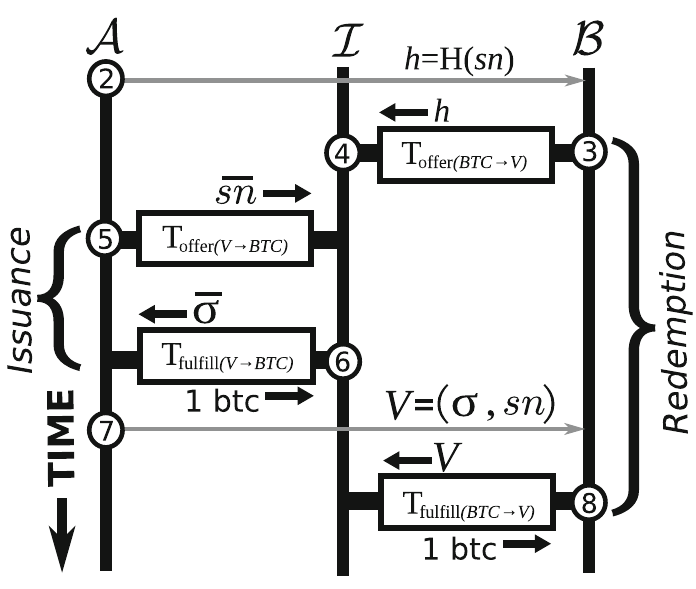
\includegraphics[width=0.6\linewidth]{img/ecash-scheme.png}
	\caption{Scheme of how a mixing service works}
	\label{fig:mixing-service-scheme}
\end{figure}
